% Provenance (never printed): old seconde/premiere S material on soil as a
% slowly renewed resource (alteration of rocks, clays, the clay--humus
% complex, soil erosion); see sources/book2/PROVENANCE.md. Rates are the
% medians of Montgomery (2007), computed in figdata/grade-10/soil_rates.py.
\chapter{Bodem, een hulpbron die langzaam ontstaat}\label{ch:g10:soil-formation}

Een weg die door een heuvel in de vochtige tropen is uitgegraven, toont een wand
van rode aarde, verscheidene keren zo hoog als een mens. Onderaan is het gesteente
nog herkenbaar: bleek, gestreept, maar zo zacht dat het tussen je vingers
verkruimelt, terwijl het nog de korrels en banden laat zien van het gesteente
dat het ooit was. Naar boven toe gaat het over in een gevlekte klei, dan in een
harde rode laag, dan in een dunne bodem waarin de wortels zitten. De hele wand
was ooit massief gesteente: het is het gesteente zelf, dat ter plaatse langzaam
door water en lucht is omgevormd. De bodem, waarop alle planten van het land en
het voedsel van bijna alle mensen groeien, is de top van zo'n kolom. Dit
hoofdstuk legt uit hoe gesteente bodem wordt, welke scheikunde het werk doet,
hoe het klimaat het tempo bepaalt, en waarom bodem, die zo langzaam ontstaat,
zo snel verloren kan gaan.

\begin{omfigure}
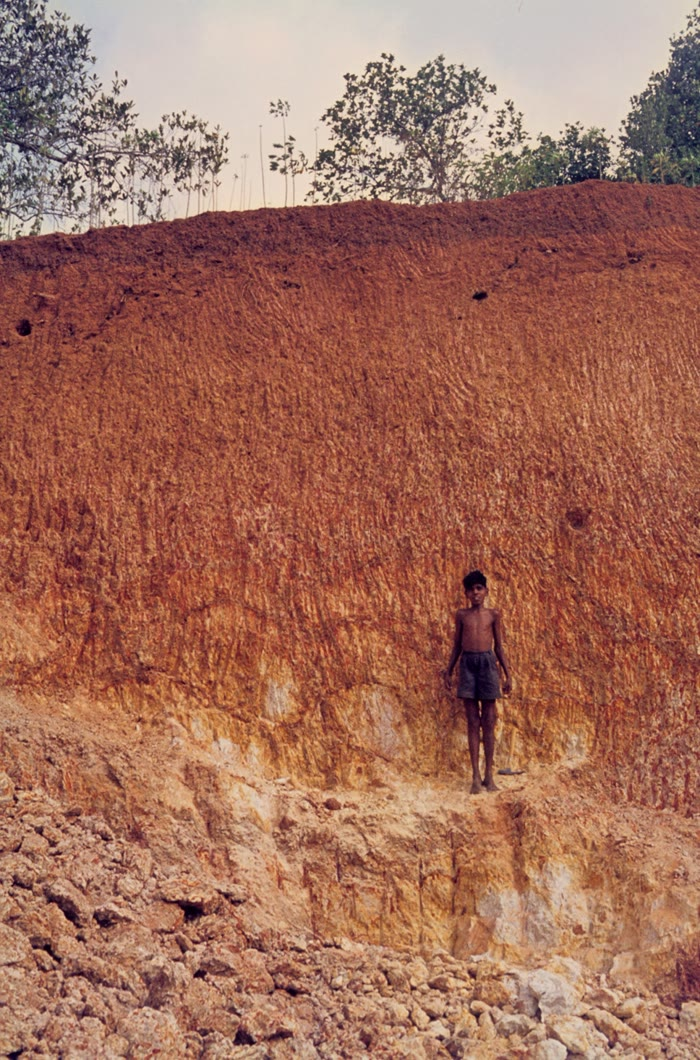
\includegraphics[height=8.5cm]{images/book2/g10-laterite-kerala.jpg}

{\small Een verweringsprofiel op granietgneis in Kerala, in het zuiden van India:
onderaan een gevlekt, ontbonden gesteente; daarboven een bruine, zwak verharde
\omterm{def:g10:soil-formation:laterite}{lateriet} onder een dunne bodem. De jongen geeft de schaal aan. Foto: Werner
Schellmann, 1969 (CC~BY-SA~2.5).}
\end{omfigure}

\begin{recall}
Verwering breekt gesteenten af waar ze liggen; erosie voert de stukken weg;
afzetting legt ze elders neer (Boek 1, jaar 5). Gesteenten bestaan uit
mineralen, zoals kwarts, veldspaten en mica's in een graniet (Boek 1, jaar
6). Een bodem is een levende laag van minerale korrels, humus, water, lucht en
organismen; afbrekers zetten dood materiaal om in humus; een bodem wordt
beschreven door zijn lagen, of horizonten (de biologieboeken). Bij een oxidatie
verliest een stof elektronen, vaak door zich met zuurstof te verbinden (de
scheikundeboeken).
\end{recall}

\section{Van gesteente tot bodem}

Fysische verwering --- vorstwerking, opwarming en afkoeling, wortels --- breekt
gesteente in stukken zonder zijn mineralen te veranderen. \omterm{def:g10:soil-formation:chemical-weathering}{Chemische verwering}
verandert de mineralen zelf. Samen veranderen ze over lange tijd de top van het
vaste gesteente in een losse mantel die naar beneden dikker wordt, naarmate de
verwering zich in het gesteente eronder vreet.

\begin{definition}[Moedergesteente; saproliet]\label{def:g10:soil-formation:weathering-profile}
Het \emph{moedergesteente}\index{moedergesteente} van een bodem is het gesteente
waaruit zijn minerale deel is ontstaan. \emph{Saproliet}\index{saproliet} is
gesteente dat ter plaatse door verwering is ontbonden: zacht en aardachtig, toont
het nog de korrels en de structuur van het moedergesteente. Een
\emph{verweringsprofiel} is de hele kolom van het verse gesteente, via de
saproliet, tot de bodem bovenaan.
\end{definition}
% ledger: usgs:saprolite

\omterm{def:g10:soil-formation:weathering-profile}{Saproliet} kan dik zijn. Onder de glooiende heuvels langs de oostkant van de
Appalachen, in het oosten van de Verenigde Staten, bereikt hij plaatselijk
ongeveer \qty{46}{m} (150 voet), al verschilt zijn dikte sterk van plaats tot
plaats; de bodem is er alleen het bovenste deel van.
% ledger: usgs:saprolite

\begin{omfigure}
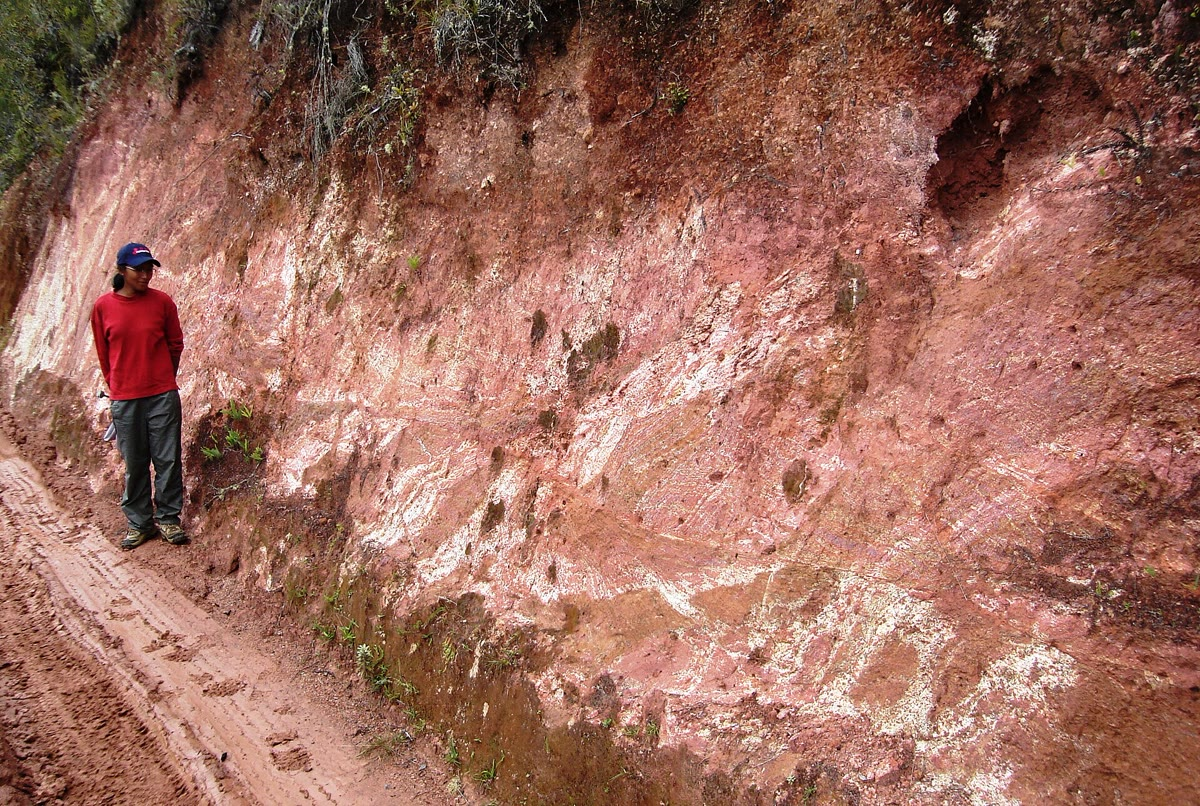
\includegraphics[width=0.8\linewidth]{images/book2/g10-saprolite-madagascar.jpg}

{\small \omterm{def:g10:soil-formation:weathering-profile}{Saproliet} in een weginsnijding in het midden van Madagaskar: de oude
gneis, ter plaatse ontbonden, toont zijn banden nog als strepen witte klei in
rode aarde. Foto: Diorit (CC~BY-SA~3.0).}
\end{omfigure}

\begin{omfigure}
\begin{tikzpicture}[font=\footnotesize]
  % humid tropical column
  \begin{scope}
    \fill[omThm!45!brown!60] (0,5.4) rectangle (1.8,6.0);
    \fill[omThm!70!orange!70] (0,4.2) rectangle (1.8,5.4);
    \fill[omThm!25!orange!35] (0,1.2) rectangle (1.8,4.2);
    \foreach \y in {1.5,2.1,2.7,3.3,3.9} \draw[white!80!black, thick] (0.1,\y) -- (1.7,\y+0.15);
    \fill[black!30] (0,0) rectangle (1.8,1.2);
    \foreach \x/\y in {0.3/0.3,0.9/0.7,1.4/0.2,0.5/0.9,1.2/1.0} \draw[black!55] (\x,\y) -- ++(0.2,0.08);
    \draw[black!60] (0,0) rectangle (1.8,6.0);
    \node[anchor=north, align=center] at (0.9,-0.1) {vochtige tropen};
  \end{scope}
  % temperate column
  \begin{scope}[xshift=3.2cm]
    \fill[omThm!45!brown!60] (0,2.2) rectangle (1.8,2.6);
    \fill[omThm!25!orange!35] (0,1.2) rectangle (1.8,2.2);
    \foreach \y in {1.5,1.9} \draw[white!80!black, thick] (0.1,\y) -- (1.7,\y+0.15);
    \fill[black!30] (0,0) rectangle (1.8,1.2);
    \foreach \x/\y in {0.3/0.3,0.9/0.7,1.4/0.2,0.5/0.9,1.2/1.0} \draw[black!55] (\x,\y) -- ++(0.2,0.08);
    \draw[black!60] (0,0) rectangle (1.8,2.6);
    \node[anchor=north, align=center] at (0.9,-0.1) {gematigd\\klimaat};
  \end{scope}
  % labels
  \draw[black!50] (5.3,5.7) -- (2.0,5.7); \node[anchor=west] at (5.4,5.7) {bodem};
  \draw[black!50] (5.3,4.8) -- (2.0,4.8); \node[anchor=west, align=left] at (5.4,4.8) {lateriet: rood, rijk aan ijzer-\\en aluminiumoxiden};
  \draw[black!50] (5.3,3.4) -- (2.0,3.4); \node[anchor=west, align=left] at (5.4,3.4) {saproliet: ter plaatse ontbonden\\gesteente, structuur behouden};
  \draw[black!50] (5.3,0.6) -- (5.0,0.6); \node[anchor=west] at (5.4,0.6) {vers moedergesteente};
\end{tikzpicture}

{\small Twee verweringsprofielen op hetzelfde gesteente (schematisch, niet op
schaal): onder een heet, nat klimaat is het profiel veel dikker en is de top een
\omterm{def:g10:soil-formation:laterite}{lateriet}; onder een gematigd klimaat draagt een dunnere \omterm{def:g10:soil-formation:weathering-profile}{saproliet} de bodem.}
\end{omfigure}

\section{Chemische verwering}

\begin{definition}[Chemische verwering]\label{def:g10:soil-formation:chemical-weathering}
\emph{Chemische verwering}\index{chemische verwering} is de omvorming van de
mineralen van een gesteente door reacties met water en met de gassen die het
meevoert, koolstofdioxide en zuurstof: sommige mineralen lossen op, andere worden
omgezet in nieuwe mineralen, die stabiel zijn aan het aardoppervlak.
\end{definition}

Regenwater neemt een beetje koolstofdioxide uit de lucht op, en veel meer
wanneer het door de bodem sijpelt, waar wortels en afbrekers het uitademen. Een
deel van het opgeloste gas vormt koolzuur, dat waterstofionen vrijmaakt:
\begin{center}
\ce{CO2 + H2O -> H+ + HCO3-}
\end{center}
Deze waterstofionen tasten de mineralen aan.

\begin{definition}[Hydrolyse]\label{def:g10:soil-formation:hydrolysis}
\emph{Hydrolyse}\index{hydrolyse} is de \omterm{def:g10:soil-formation:chemical-weathering}{chemische verwering} van een
silicaatmineraal door water en zijn waterstofionen: de waterstofionen nemen de
plaats in van de metaalionen van het mineraal, die in oplossing gaan, en de rest
van het mineraal wordt omgebouwd tot een \omterm{def:g10:soil-formation:clay}{kleimineraal}.
\end{definition}

\begin{proposition}[Hydrolyse van een veldspaat]\label{prop:g10:soil-formation:hydrolysis}
De kaliveldspaat orthoklaas, \ce{KAlSi3O8}, wordt door \omterm{def:g10:soil-formation:hydrolysis}{hydrolyse} omgezet in het
\omterm{def:g10:soil-formation:clay}{kleimineraal} kaoliniet, \ce{Al2Si2O5(OH)4}; kaliumionen en opgelost silica,
\ce{H4SiO4}, worden door het water afgevoerd:
\begin{center}
\ce{2 KAlSi3O8 + 2 H+ + 9 H2O -> Al2Si2O5(OH)4 + 2 K+ + 4 H4SiO4}
\end{center}
\end{proposition}
% ledger: webmineral:formulas

\begin{proof}[Controle]
Tel elk element aan beide kanten. Kalium: 2 en 2. Aluminium: 2 en 2.
Silicium: 6 en $2 + 4 = 6$. Zuurstof: $16 + 9 = 25$ en $9 + 16 = 25$.
Waterstof: $2 + 18 = 20$ en $4 + 16 = 20$. Lading: $+2$ en $+2$.
\end{proof}

\begin{proposition}[Oplossen van calciet]\label{prop:g10:soil-formation:calcite}
Calciet, \ce{CaCO3}, het mineraal van kalksteen, lost volledig op in water dat
koolstofdioxide meevoert; er blijft niets vasts over:
\begin{center}
\ce{CaCO3 + CO2 + H2O -> Ca^2+ + 2 HCO3-}
\end{center}
\end{proposition}
% ledger: webmineral:formulas

IJzer wordt op een derde manier aangetast. In de donkere mineralen van een
gesteente, zoals de zwarte mica van een graniet, zit ijzer in de gereduceerde
vorm \ce{Fe^2+}. Zuurstof die met het water wordt meegevoerd, oxideert het, en
het ijzer(III) blijft achter als onoplosbare oxiden: geelbruin goethiet,
\ce{FeO(OH)}, en rood hematiet, \ce{Fe2O3}. Voor goethiet:
\begin{center}
\ce{4 Fe^2+ + O2 + 6 H2O -> 4 FeO(OH) + 8 H+}
\end{center}
Deze oxiden kleuren verweerde gesteenten en bodems geel, bruin en rood.
% ledger: webmineral:formulas

Niet alle mineralen verweren in hetzelfde tempo. In een verwerend graniet roest
de zwarte mica en worden de veldspaten klei, maar de kwartskorrels, bijna
onoplosbaar, komen er onveranderd uit: ze eindigen als zand.

\begin{example}[De verwering van een graniet]\label{ex:g10:soil-formation:granite}
% ledger: webmineral:formulas (masses computed in figdata/grade-10/soil_rates.py)
Een kilogram orthoklaas bevat $1000/278.33 \approx \qty{3.59}{mol}$
\ce{KAlSi3O8}. Volgens de vergelijking geven twee mol orthoklaas één mol
kaoliniet: $3.59/2 \approx \qty{1.80}{mol}$, dat is $1.80 \times 258.16
\approx \qty{464}{g}$ klei. Het kalium, $14.05~\%$ van de massa van het
orthoklaas, \qty{140.5}{g}, en $2 \times 3.59 = \qty{7.19}{mol}$ silica
gaan in oplossing weg. Uit een graniet van kwarts, veldspaten en mica's laat de
verwering zand (het kwarts), klei (uit de veldspaten en mica's) en ijzeroxiden
achter, en stuurt ze kalium, natrium, calcium en silica naar de rivieren.
\end{example}

\section{Klei en humus}

\begin{definition}[Kleimineraal]\label{def:g10:soil-formation:clay}
Een \emph{kleimineraal}\index{kleimineraal} is een silicaat dat is opgebouwd uit
dunne lagen atomen die op elkaar gestapeld zijn, gevormd door verwering, en dat
voorkomt als schilfers die veel kleiner zijn dan zandkorrels. Kaoliniet is er een van.
\end{definition}
% ledger: webmineral:formulas

De oppervlakken van kleischilfers dragen negatieve elektrische ladingen. Ze
houden positieve ionen vast --- kalium \ce{K+}, calcium \ce{Ca^2+}, magnesium
\ce{Mg^2+}, ammonium \ce{NH4+} --- die anders door de regen zouden worden
weggespoeld. Humus doet hetzelfde. Samen vormen klei en humus het
\emph{klei-humuscomplex}, de voorraad minerale voedingsstoffen van de bodem: een
wortel geeft waterstofionen af en neemt in ruil het kalium of calcium op dat op
de schilfers is vastgehouden.

\begin{omfigure}
\begin{tikzpicture}[font=\footnotesize, >={Stealth[length=2mm]}]
  \foreach \y in {0,0.7,1.4} {
    \fill[omExo!35, draw=black!60] (0,\y) rectangle (7.2,\y+0.3);
    \foreach \x in {0.3,0.9,...,7.0} \node[font=\tiny, black!70] at (\x,\y+0.15) {$-$};
  }
  \foreach \x/\ion in {0.7/K^+, 1.9/Ca^{2+}, 3.1/K^+, 4.3/Mg^{2+}, 5.5/NH_4^+, 6.7/K^+} {
    \fill[omThm!20, draw=omThm!80!black] (\x,2.1) circle (0.4);
    \node[font=\scriptsize] at (\x,2.1) {$\mathrm{\ion}$};
  }
  \foreach \x in {1.3, 3.7, 6.1} \fill[omThm!20, draw=omThm!80!black] (\x,0.5) circle (0.17);
  \foreach \x in {2.5, 4.9} \fill[omThm!20, draw=omThm!80!black] (\x,1.2) circle (0.17);
  \node[anchor=north] at (3.6,-0.1) {kleilagen, negatief geladen, met positieve ionen ertussen};
  \node[anchor=south] at (3.1,2.5) {positieve ionen vastgehouden op de oppervlakken};
  % root and exchange
  \draw[line width=2.2pt, brown!60!black] (9.6,3.4) .. controls (9.3,2.6) and (8.9,2.2) .. (8.1,2.0);
  \node[anchor=east] at (9.25,3.3) {wortel};
  \draw[->, omDef!80!black, thick] (8.0,2.2) .. controls (7.6,2.6) and (7.2,2.6) .. (6.95,2.3);
  \node[anchor=south, omDef!80!black] at (7.5,2.55) {\ce{H+} afgegeven};
  \draw[->, omThm!80!black, thick] (6.95,1.8) .. controls (7.3,1.5) and (7.7,1.6) .. (8.0,1.85);
  \node[anchor=north, omThm!80!black] at (7.8,1.55) {\ce{K+} opgenomen};
\end{tikzpicture}

{\small Het klei-humuscomplex (schematisch): negatief geladen kleilagen houden
positieve ionen vast op hun oppervlakken en ertussen; een wortel ruilt
waterstofionen voor deze voedingsstoffen.}
\end{omfigure}

\section{Bodems en klimaat}

\omterm{def:g10:soil-formation:chemical-weathering}{Chemische verwering} heeft water nodig, en zoals de meeste reacties verloopt ze
sneller wanneer het warm is. Waar het klimaat zowel heet als nat is, wordt
gesteente het diepst en het verst ontbonden: de veldspaten worden volledig klei,
zelfs een groot deel van het silica wordt afgevoerd, en wat overblijft is rijk aan
de minst oplosbare elementen, ijzer en aluminium.

\begin{definition}[Lateriet]\label{def:g10:soil-formation:laterite}
Een \emph{lateriet}\index{lateriet} is een diep verweerd materiaal van hete,
natte klimaten, rood of bruin, dat vooral bestaat uit ijzer- en aluminiumoxiden en
kaoliniet, en waaruit bijna alles wat oplosbaar is, is verwijderd.
\end{definition}

Onder koude klimaten, die een groot deel van het jaar bevroren zijn, en onder
droge klimaten, waar water schaars is, verloopt \omterm{def:g10:soil-formation:chemical-weathering}{chemische verwering} langzaam: de
bodems zijn dun en het gesteente ligt er vlak onder. Tussen de polen en de
evenaar is de verweringsdiepte het grootst onder de vochtige tropische bossen en
het kleinst in de woestijnen en de poolgebieden.

\begin{omfigure}
\begin{tikzpicture}[font=\footnotesize]
  \fill[black!25] (0,-0.2) -- (0,-0.5) .. controls (1.5,-0.6) and (2.5,-1.4) .. (3.4,-1.2)
     .. controls (4.2,-1.0) and (4.6,-0.55) .. (5.2,-0.5) .. controls (6.0,-0.5) and (6.6,-1.6) .. (7.6,-3.0)
     .. controls (8.2,-3.6) and (9.0,-3.6) .. (10,-3.4) -- (10,-3.8) -- (0,-3.8) -- cycle;
  \fill[omThm!25!orange!35] (0,0) -- (10,0) -- (10,-3.4) .. controls (9.0,-3.6) and (8.2,-3.6) .. (7.6,-3.0)
     .. controls (6.6,-1.6) and (6.0,-0.5) .. (5.2,-0.5) .. controls (4.6,-0.55) and (4.2,-1.0) .. (3.4,-1.2)
     .. controls (2.5,-1.4) and (1.5,-0.6) .. (0,-0.5) -- cycle;
  \draw[black!60] (0,0) -- (10,0);
  \node[anchor=south] at (0.6,0.05) {polair};
  \node[anchor=south] at (3.2,0.05) {gematigd};
  \node[anchor=south] at (5.3,0.05) {woestijn};
  \node[anchor=south] at (6.8,0.05) {savanne};
  \node[anchor=south] at (9.0,0.05) {tropisch bos};
  \node[anchor=north] at (0.4,-3.85) {pool};
  \node[anchor=north] at (9.6,-3.85) {evenaar};
  \node[black!70] at (2.0,-2.6) {vers gesteente};
  \node[black!80] at (8.35,-1.0) {verweerd gesteente en bodem};
\end{tikzpicture}

{\small De verweringsdiepte van een pool tot de evenaar (schematisch, diepten
niet op schaal): klein onder polaire en woestijnklimaten, middelmatig onder
gematigde klimaten, het grootst onder de vochtige tropische bossen.}
\end{omfigure}

\section{Langzaam gevormd, snel verloren}

Hoe snel ontstaat bodem? De bodemproductie, de snelheid waarmee verwering aan de
basis van het profiel gesteente in bodem omzet, is op veel plaatsen in de wereld
gemeten, en ook de snelheid waarmee bodem aan het oppervlak wordt weggeërodeerd.
Een verzameling van deze metingen geeft de typische (mediane) snelheden
hieronder, elk uitgedrukt als een dikte bodem per jaar.
% ledger: montgomery:rates

\begin{omfigure}
\begin{tikzpicture}
\begin{axis}[omrecord, width=0.82\linewidth, height=5.6cm, ymode=log, log origin=infty, ymin=0.005,
  ymax=5, ybar, bar width=16pt, xtick={0,1,2,3,4}, xmin=-0.6, xmax=4.6,
  xticklabels={{bodem-\\productie}, {erosie onder\\natuurlijke begroeiing}, {geologische\\erosie}, {conserverende\\landbouw}, {conventioneel\\ploegen}},
  xticklabel style={align=center, font=\scriptsize},
  ylabel={snelheid (\unit{mm} per jaar)}, tick label style={font=\small}, label style={font=\small},
  nodes near coords, nodes near coords style={font=\scriptsize}, point meta=explicit symbolic]
\addplot[fill=omDef!45, draw=omDef!80!black] table[x=idx, y=rate_mm_yr, meta=rate_mm_yr] {figdata/out/grade-10-soil_rates-rates.dat};
\end{axis}
\end{tikzpicture}

{\small Mediane snelheden van bodemproductie en van erosie uit een wereldwijde
verzameling metingen, in millimeter bodem per jaar (logaritmische schaal: elke
stap is tien keer de stap eronder).
Gegevens: Montgomery (2007), \emph{Proceedings of the National Academy of Sciences}.}
\end{omfigure}
% ledger: montgomery:rates

Onder natuurlijke begroeiing erodeert bodem ongeveer even snel als hij ontstaat,
rond \qty{0.02}{mm} per jaar: een centimeter in zo'n zes eeuwen. Bij
conventioneel ploegen, dat de grond tussen de teelten kaal laat, is de mediane
erosiesnelheid \qty{1.5}{mm} per jaar, negentig keer de bodemproductie. Bij
conserverende landbouw, die de bodem minder verstoort en bedekt houdt, daalt de
mediaan tot \qty{0.08}{mm} per jaar, veel dichter bij de snelheid van de
productie.
% ledger: montgomery:rates (ratios computed in figdata/grade-10/soil_rates.py)

\begin{method}[Een vormingssnelheid vergelijken met een erosiesnelheid]\label{met:g10:soil-formation:rates}
\begin{enumerate}
  \item Druk beide snelheden uit in dezelfde eenheid (millimeter per jaar).
  \item Het nettoverlies is de erosiesnelheid $E$ min de productiesnelheid $P$.
  \item Een bodem met dikte $S$ gaat verloren in $T = S/(E - P)$ jaar; als
        $E \le P$, gaat de bodem niet verloren.
  \item Om vanaf nul een dikte $S$ te vormen, zijn $S/P$ jaren nodig.
\end{enumerate}
\end{method}
% ledger: montgomery:lifetime

Met deze snelheden duurt het ongeveer $1000/0.017 \approx 59\,000$ jaar om een
meter bodem te vormen, en bij conventioneel ploegen kan die in ongeveer
$1000/(1.537 - 0.017) \approx 660$ jaar verloren gaan. Op de tijdschaal van
mensen is bodem een hulpbron die zich niet vernieuwt.
% ledger: montgomery:rates, montgomery:lifetime

\begin{omfigure}
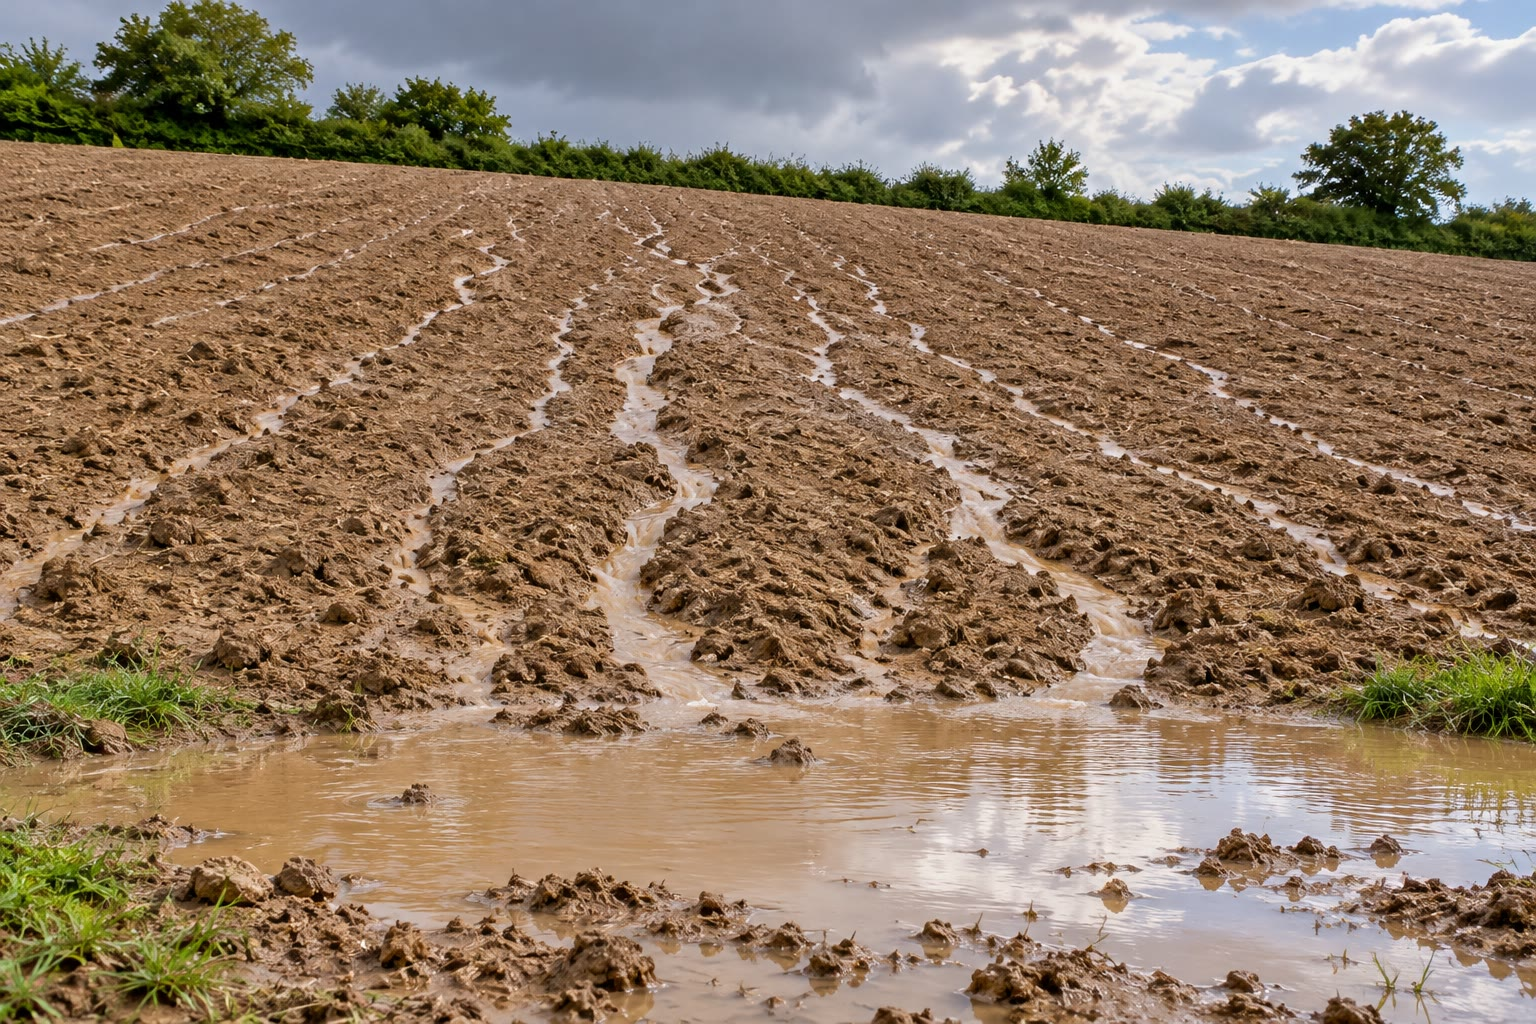
\includegraphics[width=0.72\linewidth]{images/book2/ai/g10-ploughed-rills.jpg}

{\small Een geploegde akker na een zware stortbui: het afstromende water heeft
kleine geulen, of rills, in de helling uitgesneden en de bodem meegevoerd naar
een modderige plas aan de voet ervan.}
\end{omfigure}

\section{Oefeningen}

\begin{exercise}[$\star$]\label{exo:g10:soil-formation:1}
Definieer \omterm{def:g10:soil-formation:chemical-weathering}{chemische verwering} en \omterm{def:g10:soil-formation:hydrolysis}{hydrolyse}.
\end{exercise}

\begin{exercise}[$\star$]\label{exo:g10:soil-formation:2}
Wat is \omterm{def:g10:soil-formation:weathering-profile}{saproliet}? Hoe onderscheid je \omterm{def:g10:soil-formation:weathering-profile}{saproliet} van een bodem die is gevormd in
zand dat door een rivier is aangevoerd?
\end{exercise}

\begin{exercise}[$\star$]\label{exo:g10:soil-formation:3}
Noem de producten van de verwering van een graniet: wat wordt elk van zijn drie
belangrijkste mineralen?
\end{exercise}

\begin{exercise}[$\star$]\label{exo:g10:soil-formation:4}
Waarom zijn verweerde gesteenten en tropische bodems zo vaak rood, geel of bruin?
\end{exercise}

\begin{exercise}[$\star$]\label{exo:g10:soil-formation:5}
Geef met behulp van het staafdiagram de mediane bodemproductie en de mediane
erosiesnelheid bij conventioneel ploegen. Hoeveel keer groter is de
tweede?
\end{exercise}

\begin{exercise}[$\star\star$]\label{exo:g10:soil-formation:6}
Ga na dat de vergelijking van het oplossen van calciet klopt, voor elk element
en voor de lading.
\end{exercise}

\begin{exercise}[$\star\star$]\label{exo:g10:soil-formation:7}
Kalksteen lost volledig op, graniet laat zand en klei achter. Verklaar het
verschil met de twee reacties uit het hoofdstuk.
\end{exercise}

\begin{exercise}[$\star\star$]\label{exo:g10:soil-formation:8}
Leg uit hoe het klei-humuscomplex kalium vasthoudt in een bodem waar de regen
doorheen spoelt, en hoe een wortel het opneemt.
\end{exercise}

\begin{exercise}[$\star\star$]\label{exo:g10:soil-formation:9}
Geef twee redenen waarom \omterm{def:g10:soil-formation:laterite}{laterieten} ontstaan onder hete, natte klimaten en niet
onder koude of droge.
\end{exercise}

\begin{exercise}[$\star\star$]\label{exo:g10:soil-formation:10}
De mediane bodemproductie is \qty{0.017}{mm} per jaar. Hoe lang duurt het om
\qty{1}{cm}, \qty{30}{cm} en \qty{1}{m} bodem te vormen?
\end{exercise}

\begin{exercise}[$\star\star$]\label{exo:g10:soil-formation:11}
Erosiesnelheden worden vaak gegeven als een massa bodem per hectare per jaar.
Welke massa stelt een verlies van \qty{1.5}{mm} per jaar voor op één hectare
(\qty{10000}{m^2}), bij een dichtheid van de bodem van \qty{1200}{kg/m^3}?
\end{exercise}

\begin{exercise}[$\star\star\star$]\label{exo:g10:soil-formation:12}
Onder de heuvels van een gematigd gebied is \omterm{def:g10:soil-formation:weathering-profile}{saproliet} van \qty{46}{m} dik
ontstaan. Als de verwering met \qty{0.017}{mm} per jaar in het gesteente
voortschreed, hoe lang zou dat dan hebben geduurd? Wat zegt het antwoord over de
ouderdom van zo'n landschap?
\end{exercise}

\begin{exercise}[$\star\star\star$]\label{exo:g10:soil-formation:13}
Schrijf de vergelijking van de oxidatie van \ce{Fe^2+} tot goethiet uit het
hoofdstuk op en controleer ze. Schrijf daarna de oxidatie van \ce{Fe^2+} tot
hematiet, \ce{Fe2O3}, door zuurstof en water, waarbij \ce{H+} vrijkomt, en maak ze kloppend.
\end{exercise}

\begin{exercise}[$\star\star\star$]\label{exo:g10:soil-formation:14}
Bij conserverende landbouw is de mediane erosiesnelheid \qty{0.082}{mm} per
jaar. Hoe lang duurt het, met een bodemproductie van \qty{0.017}{mm} per jaar,
om \qty{30}{cm} bodem te verliezen? Vergelijk met conventioneel ploegen.
\end{exercise}

\begin{exercise}[$\star\star\star$]\label{exo:g10:soil-formation:15}
Een graniet bevat \qty{30}{\percent} orthoklaas naar massa. Welke massa kaoliniet
ontstaat er wanneer al het orthoklaas van één ton van dit graniet is verweerd, en
welke massa kalium komt er vrij?
\end{exercise}

\section{Probleem: de levensduur van een bodem}

\begin{problem}[{Weekendprobleem --- van gesteente tot akker en terug naar de rivier}]
\label{pb:g10:soil-formation:1}
% ledger: montgomery:rates, montgomery:lifetime, webmineral:formulas (values computed in figdata/grade-10/soil_rates.py)

\begin{center}
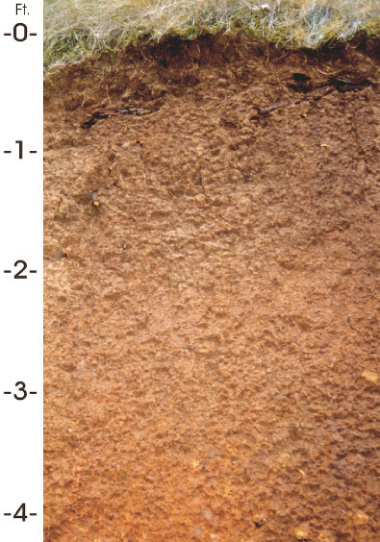
\includegraphics[height=6cm]{images/book2/g10-nrcs-jory-soil.jpg}

{\small Een bodemprofiel, met links een schaal in voet (\num{1}~voet =
\qty{0.3048}{m}). Foto: USDA Natural Resources Conservation Service
(publiek domein).}
\end{center}

\medskip
\noindent\textbf{Deel I --- Een profiel.}
\begin{enumerate}
  \item De schaal reikt tot 4 voet bij de onderkant van de foto. Hoe diep is
        dat, in meter?
  \item De donkere laag bovenaan reikt tot ongeveer een halve voet. Hoe dik is
        ze, in centimeter?
  \item Wat geeft deze bovenste laag haar donkere kleur?
  \item Daaronder is de bodem roodbruin. Welke mineralen geven hem deze kleur, en
        hoe zijn ze ontstaan?
  \item Is het \omterm{def:g10:soil-formation:weathering-profile}{moedergesteente} op de foto zichtbaar? Wat zou je verwachten onder
        de onderkant van de foto aan te treffen?
\end{enumerate}

\medskip
\noindent\textbf{Deel II --- De scheikunde van een verwerend graniet.}
\begin{enumerate}[resume]
  \item Schrijf de vergelijking van de \omterm{def:g10:soil-formation:hydrolysis}{hydrolyse} van orthoklaas op.
  \item Hoeveel mol orthoklaas zit er in \qty{1}{kg}
        (\qty{278.33}{g/mol})?
  \item Welke massa kaoliniet (\qty{258.16}{g/mol}) leveren ze?
  \item Wat gaat er met het water weg, en waar gaat het naartoe?
  \item Wat gebeurt er met het kwarts van het graniet?
\end{enumerate}

\medskip
\noindent\textbf{Deel III --- Vorming tegenover erosie.}
\begin{enumerate}[resume]
  \item Bodem ontstaat met \qty{0.017}{mm} per jaar. Hoe lang duurt het om het
        profiel van deel I te vormen?
  \item Bij conventioneel ploegen erodeert bodem met \qty{1.537}{mm} per
        jaar. Wat is het nettoverlies per jaar?
  \item Hoe lang zou het profiel van deel I meegaan?
  \item Vergelijk de twee tijden van de vragen 11 en 13.
  \item Onder natuurlijke begroeiing is de erosie \qty{0.013}{mm} per jaar. Gaat
        de bodem verloren?
\end{enumerate}

\medskip
\noindent\textbf{Deel IV --- De levensduur van de bodem.}
\begin{enumerate}[resume]
  \item Schrijf de tijd $T$ om een dikte $S$ bodem te verliezen als functie van
        $S$, van de erosiesnelheid $E$ en van de productiesnelheid $P$.
  \item Bereken $T$ voor $S = \qty{30}{cm}$ bij conventioneel ploegen.
  \item Bereken $T$ voor $S = \qty{30}{cm}$ bij conserverende landbouw
        (\qty{0.082}{mm} per jaar).
  \item Waarom kun je een bodem een hulpbron noemen die zich op de tijdschaal van
        mensen niet vernieuwt?
  \item Hoe lang duurt het om bij conventioneel ploegen een meter bodem te
        verliezen?
\end{enumerate}
\end{problem}
